\subsection{Product perspective}
\subsubsection{Scenarios}
\begin{enumerate}[label=\textbf{\arabic*}.]
    \item \textbf{ Educator creates a tournament}\\Alan is a university professor. He has just finished explaining a very hard topic that occupied multiple lectures. He would like to test its class about it but exams dates are far away ahead and he thinks that trying to evaluate their understanding with a quick quiz performed in class before or after his next lecture would not be a good idea given the depth of the topic. Anyway he knows of a site that allows educators to easily organize challenges to which students can take part and decides to give it a try.\\He connects to the website of the platform and signs up as an educator. After that, he navigates to the “Tournaments” section and selects the option to create a new one: inputs the name of the tournament and a deadline for the subscription. All students subscribed to the CKB platform are now notified and can join the tournament.\\Since Alan’s schedule is often very busy, he then decides to grant the permission to create battles to his teaching assistant Thomas, which has already subscribed to the platform.
    \item \textbf{ Educator creates a battle}\\Linus is a famous youtuber that publishes video courses on programming languages. He wants to increase the engagement with his subscribers, so for this reason he has already subscribed to the CKB platform and created a tournament. In his last video lecture, he has started a new playlist on Java language, explaining some basic concepts typical of object oriented programming.\\To challenge his viewers, he decides to create a new coding battle. He now connects to the website of the platform and log-ins with his credential. He clicks on the tournament called “LinusTechChallenges” he previously created and selects the option to generate a new battle. The platform then asks him to specify some settings for this specific challenge: he selects “Java” as programming language, uploads the “code kata” which includes a textual description of the challenge and all the files related to the software project like test cases and build automation scripts, selects set the minimum and maximum number of students per group, fixes the registration and final submission deadlines. Since he has many subscribers and cannot manually review every solution, he also specifies that a final manual evaluation is not needed. However, Linus decides to enable all the available aspects the static analysis should focus on (e.g. security, reliability, maintainability). At this point he confirms the creation of the battle and the system automatically notifies all the students subscribed to the tournament about the new coding battle.
    \item \textbf{ Student subscribes to a tournament}\\Mark is struggling to keep the pace of its professor’s lectures. Moreover, since his anxiety always penalizes him, he is afraid he will organize some activity in class to evaluate his knowledge about the last, complex topic. One day, while looking at the academic mail, he notices that the feared professor is contacting its students to inform them of an alternative evaluation method that would allow them to avoid part of the final exam and which involves to write code to solve problems related with the subject and compete with other students. Mark immediately decides to go for it and subscribes (as a student) to the platform indicated by the professor. Once logged in, he goes to the “Tournaments” section and selects the option to search for a specific tournament: at this point he searches the tournament by the name communicated by the professor, selects it and subscribes to it. Once a new battle will be available, he will be notified by the system. He is now ready to participate to the battles and prove what he has learned.
    \item \textbf{ Students form a team}\\Liam is a software engineer that has subscribed to CKB because a famous IT company is offering some job positions to the most talented developers discovered through the platform. For this reason, he already joined the tournament created by the company. Since the company is interested in developers with the ability to work in teams, its human resources department has set “2” as minimum number of team members for their first battle. So, Liam decides to tackle the first challenge with a trusted former university colleague of his. He navigates to the “Tournaments” section, searches and selects the ongoing tournament of the company and clicks on the first battle called “Challenge 1”. The system shows 2 options: “Create a team” and “Join a team”. Liam selects the first option and chooses a name for his team, checking the “private” flag option. The systems generates an invite code that he can now share privately to his friend in order to join the team.
    \item \textbf{ Student submits a solution}\\Jonas is subscribed to the CKB platform in order to participate in quizzes organized by his computer science professor. He is very happy with this kind of continual evaluation because it's a great way to understand those difficult concepts taught during theory classes and skip some exercises at the final written exam.\\When a new programming challenge is announced, Jonas gets excited to test his skills. He forms a team with two other classmates to collaborate on solving the exercise. After working hard to come up with a new solution, Jonas submits it to the CKB platform by committing the solution on their GitHub repository before the deadline. Jonas and his team mates have monitored their score during the whole battle, but are not satisfied with rank of their final submission computed with the automated evaluation.\\The next day, after the consolidation stage, Jonas is thrilled to see his final team rank near the top of the leaderboard! Indeed the professor liked a lot their innovative solution and decided to  reward them during the manual evaluation.
    \item \textbf{ Educator manually evaluates solutions}\\Oliver is an instructor and he is using CKB to evaluate the students enrolled in his online programming course. He enjoys the platform because it organizes the students’ GitHub repository in a convenient and central way. Indeed, once the submission phase ends, during the consolidation stage Oliver can select the current battle and go through the whole list of teams. For each team, the system shows the GitHub repository link and the scores related to the automated evaluation. After inspecting the code in the repo, Oliver inputs in the same page a natural number between 0 and 100 as manual evaluation score (the higher the better). Once he has finished reviewing the code of all the teams, he clicks on the “Terminate battle” field next to the current battle tab and all students involved are notified about the final mark.
\end{enumerate}

\subsubsection{Domain Class diagram}
\begin{figure}[H]
    \hspace{-98px}
    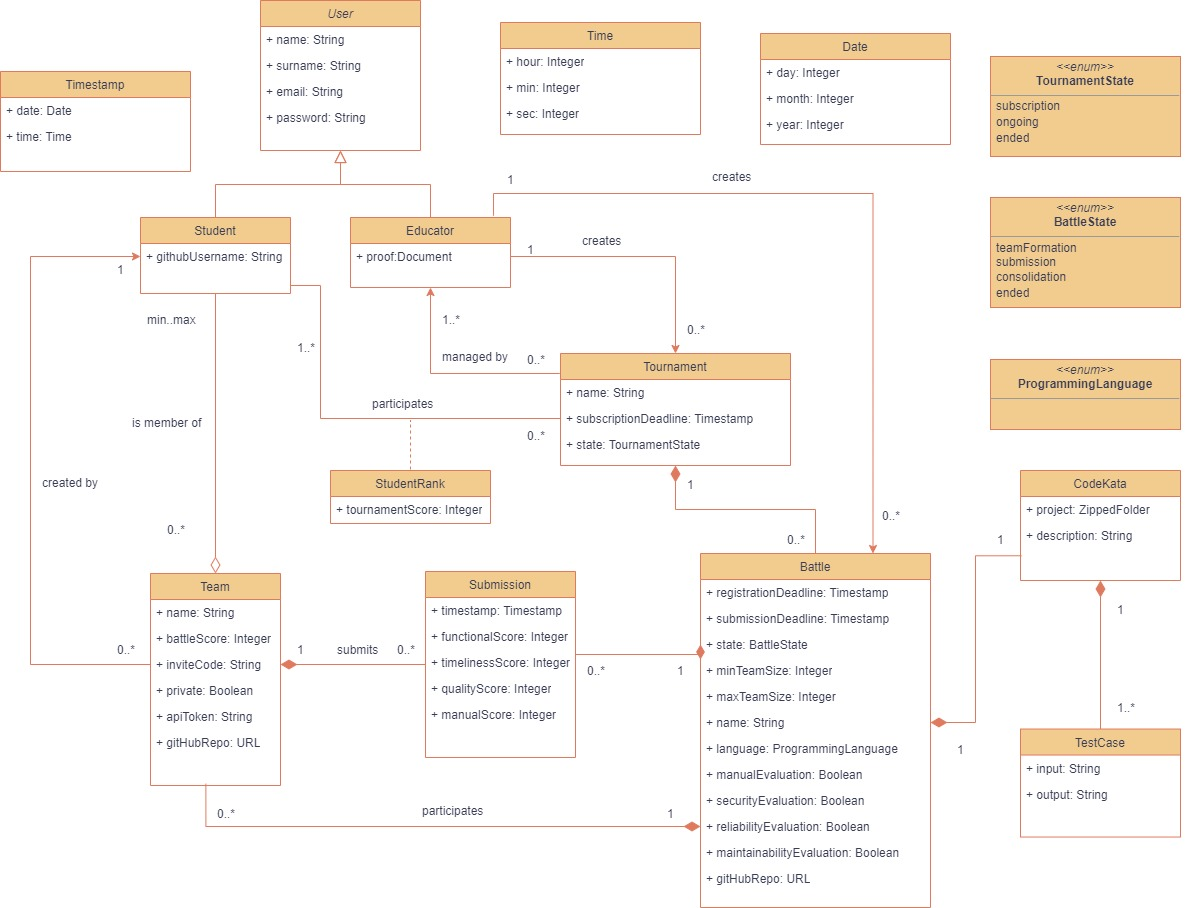
\includegraphics[scale=0.5]{Diagrams/uml_v2.jpg}
    \caption{Domain-level UML diagram}
    \label{class_diagram}
\end{figure}
\newpage
\textbf{ Additional notes on the class diagram:}
\begin{itemize}
    \item the "proofDocument" attribute of the "Educator" class contains a reference to the file through which the educator was verified. The educator verification process will not be described in this document, as it is not a functionality that directly involves the end-users of the system.
    \item the "battleScore" attribute of the Team entity contains the overall score of the latest submission. This is the score that is used to compute the rank of teams participating in the battle.
\end{itemize}

\subsubsection{State diagrams}
In order to provide a complete description of the application domain, here are included the state diagrams relative to tournaments and battles.
\begin{figure}[H]
    \hspace{-0.8cm}
    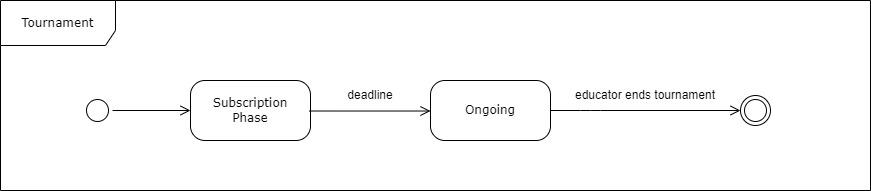
\includegraphics[scale=0.5]{Diagrams/tournament_state.jpg}
    \caption{Tournament state diagram}
    \label{tournament_state}
\end{figure}
\begin{figure}[H]
    \hspace{35px}
    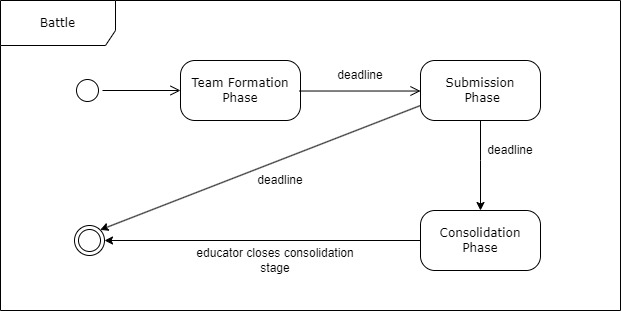
\includegraphics[scale=0.5]{Diagrams/battle_state.jpg}
    \caption{Battle state diagram}
    \label{battle_state}
\end{figure}
In particular, in the case of battles, which transition is taken after the submission stage only depends on whether the manual evaluation was enabled or not.
The Team Formation phase will be also referred to as Registration phase in the rest of the document.

\subsection{Product functions}
\subsubsection{Sign up and Log in}
These functions are used to respectively subscribe to the platform and access the personal area. This will be available to all kind of users, with a little difference between students and educators. Specifically, during the sign up process, the system will start by asking the user if he/she wants to sign up as a student or as an educator.

In the student’s case, the system will ask the new user to enter his/her first and family name, a GitHub username, an email and a password: if the provided email is not already used for another account (of any type) and it really exists a GitHub account associated to the provided username, the system registers the new user. Alternatively, the system allows users to sign up through external identity providers like Google, Facebook and GitHub.

In the educator’s case instead, the system will ask the same information but, instead of the GitHub username (which is not needed in the case of an educator), it will ask him/her a form to explain why is he/she subscribing and a document that proves its identity.

At this point, since notifications will be send via mail in any case, in order to use the system the new user has to verify its email: a verification email is sent to the provided email address containing a link that the user will have to click to confirm it.

Obviously in the future, in order to log in, the user will be asked to select the identity provider he/she originally signed up with or to provide the email and password entered during the sign up phase: if these match, the system will grant access.
\subsubsection{Manage tournaments}
This functionality is available only to educators and basically represents the main functionality that the platform provides.

In order to initiate a new competition, each educator can decide to create a new tournament. To do this the educator log in to its personal area and then goes to the page listing all the tournaments that he’s ever created (even the ones that have already terminated: the system persists their final ranks and other useful information, see “Create battles” function) or that he has been granted access to. Here the educator can click a button to create a new tournament: a new page is displayed, in which the user has to provide a new (unique) name for the tournament, fix a subscription deadline and, eventually, grant the possibility to other educators to create battles in the context of the new tournament (this is done by fulfilling a search box with their emails such that the system can send them a notification). This is the only setting that can be changed at any time, even while the tournament is active.
\subsubsection{Join a tournament}
This functionality is available only to students. In order to subscribe to a new tournament a student can find inside its personal area a page listing all the tournaments he/she has ever participated to. In this page there’s also a button that allows the student to join a new tournament: a new page is displayed, in which the user has to provide the name (or part of it) of the tournament of interest. The system searches among all the (active) tournaments those whose name is compatible with what the user’s query and returns the list of these.

At this point the student can refine his/her search or select the right tournament from the list and, by doing this, subscribe to it.
\subsubsection{Create a battle}
This functionality is available only to educators. An educator can select an active tournament from the page showing the list of the tournaments he/she has access to: inside the new page that is displayed educators can find data relative to the tournament (e.g. the state of the tournament) and the students subscribed to it (e.g. actual ranking and list of subscribed students) and also a button that allows them to create a new code kata battle.

By clicking it, the user is brought to a new webpage in which has to provide multiple information:
\begin{itemize}
    \item Battle name
    \item Programming language of use
    \item Upload Code Kata, including project description, automation scripts and test cases
    \item Set minimum and maximum number of students per group
    \item Set registration and final submission deadline
    \item Specify scoring configuration (see “Evaluate a submission” function)
\end{itemize}
At this point the battle is created and the registration phase starts.
\subsubsection{Join a battle}
This functionality is available only to students. A student that is subscribed to a tournament is notified upon the creation of a new battle in the context of it. In the case the user is interested into participating, he/she can subscribe to it by creating a team or joining one that has already been created.

As first thing he/she has to access the page relative to the teams for that battle. This can be done in 2 ways:
\begin{itemize}
    \item Directly by clicking the link inside the email sent to notify the creation of the battle.
    \item Go to the page displaying his/her list of tournaments and select the one of the new battle: inside a new page there will be shown the actual rank and the list of battles up to the last,  the active one, which can be selected. If a user selects a battle it has already subscribed to, he/she is brought to the page devoted to its team.
\end{itemize}
Inside a new page it will be displayed the list of available teams and 2 buttons.

The first button allows the student to create a new group: upon click a new page will be shown in which the student has to fill a form to enter all the necessary information. Specifically, the student has to:
\begin{itemize}
    \item Provide a (unique) name for the team
    \item Set the visibility of the group: the creator can toggle a checkbox to specify that the team will be private
\end{itemize}
At this point the system creates 2 random strings that will be univocally associated with the newly created team:
\begin{itemize}
    \item an invite code: this will represent the only way to access private teams and, in general, an alternative way to join teams.
    \item an API token: this will be requested to be included inside the GitHub Actions workflow in order to allow the system to understand which team a solution belongs to.
\end{itemize}  
This functionality is particularly important because students that want to participate by their own, need to create a group (in order to be sure, they can set it as private and simply keep the invitation code for theirselves): anyway, this scenario is available only when the minimum number of students per group is set to 1.

The second button instead allows the student to join an already existing group: this is achieved by allowing the student to search groups by name (in case of private teams, in a following page the student will be asked to provide the right invite code) or by directly providing their invite code: if the specified group does not already contain the maximum number of students for the battle, the system adds the student to the group.

Once the registration deadline is met, the system will prepare the development environment: specifically, it will create a new public repository on the platform's GitHub account and send the relative link to the members of every team subscribed to the battle. Then, the system will need \textit{only} one member per team to fork the repository, copy the relative link on the team's settings, set up GitHub Actions and invite his/her teammates (if there are) as collaborators.
\subsubsection{Submit a solution}
Once the registration phase is over, the submission phase starts: at this point each team should have its own GitHub repository in which the code for their solutions has to be collected. GitHub Actions will enable the necessary workflow: the submission of a new solution is performed by committing and pushing over the team's repository. On a new push, an API call will notify the platform of the publication of a new solution for that team and proceed to evaluate it.
\subsubsection{Evaluate a submission}
The platform provides an automatic evaluation system that is used to score the solutions submitted by the students. Scoring is divided in 2 groups:
\begin{itemize}
    \item \textbf{Automatic evaluation}: this comprises all the aspects that are mandatory to be assessed. These are:
    \begin{itemize}
        \item Correctness, measured in terms of number of test cases solved correctly out of all.
        \item Timeliness, measured in term of time passed between the registration deadline and the last commit.
        \item Quality level: the system uses external tools to evaluate the code with respect to 3 possible aspects that are security, reliability and maintainability (educator decides which to include at battle creation time).
    \end{itemize}
    These aspects are quantified and then combined in a way to return an integer score between 0 and 100.
    \item \textbf{Manual evaluation}: this is an optional evaluation phase that educators can decide to reserve time for (must be indicated at battle creation time). Specifically, in the case the educator has specified it, as soon as the mandatory evaluation has been computed the system allows him/her to manually inspect the code provided by each team: by clicking on the name of the team inside the final rank the system displays a new page in which is shown the link to the team’s GitHub repository and a form that must be filled with an integer score between 0 and 100.\\ The final mark will be computed as the arithmetic average between the automatically assessed score and the one assigned by the educator.
\end{itemize}
\subsubsection{Visualize ranking}
At any time, any user of any kind can visualize the ranking of the tournaments/battles it was involved in by reaching the dedicated page inside their personal area and selecting the tournament/battle of interest. Battle ranks are computed considering the latest score for each team, while tournament ranks are computed considering, for each student, the sum of the scores assigned to its teams in the context of that tournament.
\subsubsection{Send notification}
The system sends notifications (by means of emails) to its users in the following cases:
\begin{itemize}
    \item on tournament creation, all the students subscribed to the platform are notified
    \item on battle creation, all the students subscribed to the tournament the new battle will belong to are notified
    \item as soon as the final battle score is available, all the students belonging to the same team are notified
    \item on tournament closure, all subscribed students are notified
\end{itemize}

\subsection{User characteristics}
\subsubsection{User types}
As previously mentioned, the system is meant to be used by 2 kind of users:
\begin{itemize}
    \item \textbf{Educators}: this is the type of users that uses the platform to create competitions. They can create tournaments and battles and, eventually, evaluate the solutions provided by students. They must have a good knowledge of how to create valid automation scripts and have a basic understanding of how to use a web browser.
    \item \textbf{Students}: these are the users that will use the platform to be evaluated or simply to take part in a competition. They can subscribe to tournaments and battles, join groups of students and submit solutions. They are required to have a good knowledge of how to properly setup a GitHub repository and of all the programming languages involved in the battles.
\end{itemize} 
\subsubsection{Educator requirements}
In order to allow for automatic recognition of all the different kinds of files that the educator has to upload, the system requires him/her to upload a zip file containing all the needed files formatted in a specific way. In this section the focus is on its content rather than the way it must be structured, which instead will be described in the Design Document. 

In particular, the zip file must contain:
\begin{itemize}
    \item a folder that contains all the files needed to build the project (e.g. source code, build automation scripts, etc.). This will basically be what the GitHub repository of the battle will contain, so it must be organized in the exact way the educator wants it to appear on GitHub.
    \item a file which contains all the test cases, expressed by means of (input, expected output) couples.
\end{itemize}
This separation also allows the system to understand which files must be uploaded on the GitHub repository and which not (i.e. test cases, since they must not be visible to students).

\subsection{Assumptions, dependencies and constraints}
\subsubsection{Domain assumptions}
\begin{enumerate}[label=$\bullet$ \textbf{D\arabic*:}]
    \item Users have access to a stable and reliable internet connection to interact with the CKB platform.
    \item Supported programming languages are limited to popular options like Java, Python and C++.
    \item Registered educators are all legitimate and verified.
    \item Educators upload correct test cases and well-structured Code Kata projects.
    \item Students are expected to engage in Code Kata Battles with integrity, without resorting to plagiarism or cheating (e.g. inviting more or different collaborators with respect to the ones inside the team).
    \item Maximum number of students per group an educator can set will always be bounded (e.g. less than 4).
    \item Every student has a GitHub account.
    \item Students will fork the Code Kata GitHub repository once ready.
    \item Students know how to setup a GitHub Actions worfkflow.
    \item Only one student per group will perform the steps needed to set-up the team's repository and the GitHub Actions workflow.
    \item Static analysis tools are able to quantify the specified code quality aspects.
    \item Students use external communication channels.
\end{enumerate}